
% File acl2010.tex
%
% Contact  jshin@csie.ncnu.edu.tw or pkoehn@inf.ed.ac.uk
%%
%% Based on the style files for ACL-IJCNLP-2009, which were, in turn,
%% based on the style files for EACL-2009 and IJCNLP-2008...

%% Based on the style files for EACL 2006 by 
%%e.agirre@ehu.es or Sergi.Balari@uab.es
%% and that of ACL 08 by Joakim Nivre and Noah Smith

\documentclass[12pt]{article}
\usepackage{acl2010}
\usepackage{times}
\usepackage{url}
\usepackage{amsmath}
%\setlength\titlebox{6.5cm}    % You can expand the title box if you
% really have to
% \usepackage[brazilian]{babel}
\usepackage[brazil]{babel}
\usepackage[utf8]{inputenc}
\usepackage{graphicx}% Include figure files
%\selectlanguage{brazil}

\title{Aplicações de Treinamento Semi-Supervisionado em Casos Bipolares de Linguagem Natural}

\author{Renato Fabbri\\
Universidade de São Paulo, São Carlos, São Paulo, Brazil\\
{renato.fabbri@gmail.com}\\
{\tt Julho de 2010}}

\begin{document}

\maketitle
\begin{abstract}
Neste trabalho a técnica de aprendizado semi-supervisionado baseada em grafos chamada \emph{Propagação de Rótulos} foi aplicada à tarefa de detecção de polaridade (sentimento negativo/positivo) em fala e texto. Para trechos de fala, obtivemos grande exito com um aumento de 20\% das classificações corretas em comparação com os resultados obtidos pela utilização de métodos de aprendizado supervisionado usuais. No caso dos textos, o ganho foi moderado, resultando em ganhos gerais de 2-3\% em comparação com os métodos mais tradicionais de aprendizado supervisionado. São explicitados os métodos em utilização pelo nosso grupo de pesquisa e váriadas formas de aprimorar o resultados.
\end{abstract}

\section{Introdução}

Transportando multiplas informações concomitantes, a fala é o recurso primário do ser humano para comunicação ~\cite{spkl,flem}. Nossa cultura é marcada pela escrita e sua reprodutilbilidade, e esta é uma versão reduzida e estática da fala natural - ao menos para os homens de cultura ocidental ~\cite{guten}. As tecnologias de comunicação revelam esta natureza e primazia, em especial com os celulares e televisores, mas também pelo rádio, o qual não tem contrapartida da expressão visual. Seu estudo é essencial para práticas interpretativas e de oratória~\cite{teatro}, sem o qual um ator ou orador dificilmente alcança o resultado que busca. Diversas patologias de natureza física, psíquica ou psicogênica, manifestam traços linguísticos e paralinguísticos discerníveis por especialistas e máquinas~\cite{dalga,interactivevoice,humanmachine,benchmark}.

Características do locutor, de sua natureza e do seu estado, podem ser capturados pela análise do que ele apresenta pela fala. A idade, o gênero, origem geográfica, escolaridade, estado emocional e até condição física podem ser discernidos com base em características verbais e prosódicas ~\cite{interactivevoice}.

\section{Base Teórica}
\subsection{Processamento de Linguagem Natural}

Por \emph{linguagem natural} entende-se linguagens utilizadas por seres humanos para a comunicação cotidiana, linguagens como o português, o inglês ou o yorubá. Em contraste com linguagens artificiais como as linguagens de programação ou a linguagem matemática, as linguagens naturais se desenvolvem de geração em geração, e são difíceis de serem entendidas como uma série de regras bem definidas.

\emph{Processamento de Linguagem Natural} (PLN) é uma ampla áerea de estudos que trata da análise e produção de textos através do computador. Envolve desde técnicas estatísticas baseadas em ocorrências de palavras ou características destas\footnote{Por exemplo o tamanho e a classe gramatical de cada palavra.} até o entendimento de colocações linguísticas no sentido de dar respostas adequadas~\cite{livro-nltk}. Nosso foco é posto na \emph{análise} de estruturas textuais, mas vale ressaltar que a \emph{produção} destas estruturas também é tema de estudo.

A utilização de tecnologias baseadas em PLN está bastante difundida. Tradutores automáticos, sumarizadores e corretores ortográficos e sintáticos são exemplos tipicamente vinculados à utilização do computador. Celulares e computadores de mão fazem uso de reconhecimento de escrita. Buscadores de web (como o Google ou o Altavista), fazem uso extensivo de técnicas de PLN para detectarem palavras-chave da página indexada.

Embora o processamento de fala possa ser entendido como uma sub-área de PLN, historicamente elas são tidas como áreas distintas que muitas vezes estão postas em conjunto. Nosso projeto abrange também o processamento de fala (o que envolve acústica), o que faz da pesquisa um estudo referente ao PLN no seu sentido mais amplo. Mesmo assim, preferimos, por razões de clareza e tradição das diferentes áreas, discernir, neste trabalho, as áreas de PLN e processamento de fala.

Tarefas associadas à área de PLN abrangem desde contagem de palavras e hifenização até responstas automáticas e tradução em tempo real ~\cite{Jurafsky}. O que distingue uma aplicação de processamento de linguas de outras aplicações de processamentos de dados é a utilização de conhecimentos linguísticos. Consideremos o programa comum em sistemas unix-like de nome \emph{wc}. Quando invocado, ele retorna o número de bytes, palavras e linhas em um dado arquivo ou conjunto de arquivos. Quanto ao retornar bytes e linhas, isso é considerado uma tarefa ordinária de processamento de dados. Ao retornar o número de palavras a rotina envolve discernir o que é uma palavra, e aí o \emph{wc} se torna um sistema de processamento de linguagem.

A seguinte divisão das categorias de conhecimento linguístico é feita tanto em teoria quanto na prática:

\begin{itemize}
  \item Fonética e Fonologia - O estudo dos sons linguísticos.

  \item Morfologia - O estudo dos componentes das palavras (e seus significados).

  \item Sintáxe - O estudo da relação estrutural entre palavras.

  \item Semântica - O estudo dos significados.

  \item Pragmática - O estudo do uso da linguagem para fins específicos.

  \item Discurso - O estudo de unidades linguísticas que envolvem conjuntos de colocações, frases, etc.
\end{itemize}

\subsection{Processamento de Fala}

A caracterização acústica de um som é usualmente feita em termos do espectro e do volume. Estaremos sempre lidando com a evolução temporal do espectro do trecho de fala, seja ele um fonema, uma palavra, um segmento associado a uma emoção ou uma gravação inteira associada a uma psicopatologia ou gênero discursivo. São possíveis inúmeras formas de retratar a evolução espectral de um som e podemos apontar questões chave através de um espectrograma.

A Figura \ref{fig:espec} é um espectrograma usual. Escolhemos uma espectrograma com traços bastante claros para fins ilustrativos. O eixo vertical se refere ao espectro e o eixo horizontal às amostras. O significado real dos valores da figura depende da taxa de amostragem. Como exemplo, podemos supor que a gravação analisada tenha sido feita em $44.1 kHz$, portanto, pela lei de Nyquist a frequência máxima representada no sinal digitalizado é de $\frac{44.1 kHz}{2} = 22.05 kHz$. Notamos que a energia está concentrada abaixo de $0.7$ no espectrograma, o que corresponde a $0.7 \: \cdot \: 22.05 kHz = 15.435kHz$. Também podemos notar que o eixo horizontal se estende até ~$120k$, portanto, dada a taxa de amostragem de $44.1 kHz$, a duração do som é de $\frac{120}{44.1} \approx 2.72$ segundos. Características mais elaboradas são obtidas pela análise das proporções entre os harmônicos mais frequentes em um dado momento (p.ex. para achar a frequência fundamental).

\begin{figure}
\begin{center}
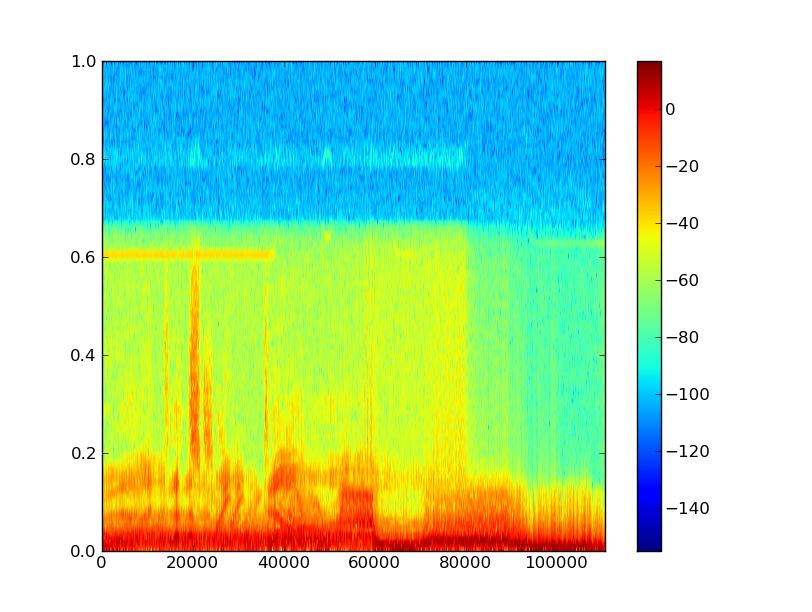
\includegraphics[scale=.4]{spec2.png}
\caption{Espectrograma padrão}
\label{fig:espec}
\end{center}
\end{figure}

Desta forma, podemos apreender características locais como a intensidade, a frequência fundamental e a proporção de harmônicos de cada \emph{grão sonoro} (duração típica entre 20-100$ms$), cada sílaba, cada palavra e cada formação contínua de fala ou construções maiores. Outras características são globais, referindo-se a cada trecho analisado. Embora existam bibliotecas disponíveis para estas tarefas, trabalhos relacionados a este Projeto muitas vezes utilizam programas como o \emph{Praat} e o \emph{WaveSurfer}, que agregam boa parte das rotinas necessárias para análises acústicas desta natureza \cite{autoreview,autoemotive}. As características extraídas são utilizadas para alimentar algum tipo de classificador de padrões como os utilizados neste trabalho.

Em geral a altura (frequência fundamental $F0$) é vista como o parâmetro mais importante para a expressão vocal de emoções. A energia (intensidade), duração e taxa de articulação são outros parâmetros relevantes. Segue uma breve descrição de cada uma destas dimensões da expressão vocal:

\begin{itemize}
\item A \emph{Frequência Fundamental} ($F0$), medida em Hertz (Hz), é a taxa com que a forma de onda se repete por unidade de tempo. A $F0$ média é a soma do valor de $F0$ para cada trecho dividida pelo número de trechos. A mediana $F0$ é o valor da $F0$ do grão que fica no meio depois da ordenação dos grãos segundo a $F0$. A $F0$ modal é o valor de $F0$ mais ocorrente no trecho em questão. É preferencialmente utilizado os percentuais 5$\,^{\circ}$ e o 95$\,^{\circ}$ em vez dos limites inferior e superior, pois tais limites podem ser ocorrências pontuais de desvios como falsetes ou perda ocasional do tônus muscular. Tais valores podem ser dados em relação à escala de semitons musicais e então o termo \emph{pitch sigma} é utilizado (a escala logarítmica é mais apropriada para pesquisas de acústica aplicadas a psicologia). A declividade da variação do $F0$ pode ser dada em semitons por segundo. É comum computar a máxima e a mínima variação de $F0$, assim como a variação média.

\item O \emph{Jitter} é definido como a variação de altura (novamente $F0$) entre ciclos consecutivos.

\item O \emph{Shimmer} é a magnitude da variação de intensidade entre ciclos consecutivos.

\item A \emph{Amplitude} é a magnitude de deslocamento de uma onda sonora, a \emph{Intensidade} se refere à quantidade de energia transmitida por unidade de tempo e o \emph{Volume} é a quantidade psicoacústica percebida da intensidade. O volume efetivo além de ser um mapeamento logarítmico da intensidade (ou da amplitude) varia também com a frequência de acordo com as curvas iso-audíveis de Fletcher-Munson. Na prática, geralmente se registra o volume somente mapeando a intensidade (ou a amplitude) para a escala logarítmica, sem adequar o volume efetivo às frequências da onda emitida.

\item A banda e a frequência média dos formantes (especialmente os primeiros três harmônicos $F1$, $F2$ e $F3$) portam informações valiosas do ponto de vista das emoções.

\item A expressão de emoções podem estar ligadas a características espectrais tais como a distribuição de frequências mais agudas. Sabemos, por exemplo, que em uma fala raivosa ou bem tensa encontramos mais harmônicos agudos (acima de $1kHz$). O oposto ocorre com fala bem relaxada ou relacionada ao tédio.

\item Quanto à \emph{Articulação}, é comum extrair os seguintes parâmetros: tempo total de fala, tempo total de pausa, tempo médio de fala, tempo médio de pausa, latência de resposta, taxa de articulação (fonemas/segundo), mínimo, máximo e desvio padrão da duração dos trechos de fala, mínimo, máximo e desvio padrão da duração dos trechos de silêncio.
\end{itemize}

Nosso trabalho está concentrado na exploração da frequência fundamental para detecção de polaridades. Salientamos que os resultados podem ser aprimorados de forma imediata simplesmente através da utilização de outras característica dos sons.

\subsection{Aprendizado Semi-supervisionado}
O \emph{aprendizado semi-supervisionado} (ASS) visa o aprendizado a partir da utilização tanto dos objetos rotulados quanto dos não rotulados. São exemplos de ASS a \emph{classificação semi-supervisionada} (CSS) e a \emph{clusterização forçada}. Este trabalho é um apanhado sobre CSS em grafos que é como geralmente é entendido o ASS com grafos.

O nome "semi-supervisionado" vem do fato de que os dados utilizados para o aprendizado está entre os dados utilizados no aprendizado supervisionado e não supervisionado\footnote{No aprendizado \emph{supervisionado} são utilizados somente dados rotulados. No aprendizado \emph{não supervisionado} são utilizados somente dados não rotulados.}.

Podemos comparar a CSS ao processo de uma criança que entende o que é um animal através de alguns exemplos dados pelos adultos e de outros vários que ela mesma observa. Ou seja, para o aprendizado do que é (e o que não é) um animal, ela utiliza tanto o conhecimento sobre os animais que contaram para ela que é um animal quanto o conhecimento sobre outros seres que não falaram para ela o que é.

Um grande atrativo dos métodos de ASS é que ele pode ajudar a contornar o fato de que os objetos rotulados podem ser custosos. Comumente necessitam de um humano especializado para rotulá-los, outras vezes necessitam de equipamentos, condições ou processamentos especiais. Muitas vezes é simplesmente impossível obter novos objetos rotulados. Já os objetos não rotulados são geralmente imediatos e abundantes, podendo ser utilizados pelo ASS de imediato.

Uma distinção importante que se faz é quanto ao ASS \emph{indutivo} e o ASS \emph{transdutivo}. O ASS indutivo se assemelha ao aprendizado transdutivo. A diferença entre ambos é que o aprendizado transdutivo é otimizado para tratar somente os objetos utilizados para o treinamento, enquanto o ASS indutivo trata de objetos não presentes na fase de treinamento.

Dados não rotulados podem ajudar de diversas formas, em especial quando as diferentes classes se mostram clusterizadas. Na Figura \ref{fig:help} é explicitado esquematicamente a forma com que os dados não rotulados podem auxiliar a determinar uma fronteira de decisão mais pertinente. Embora este seja o comportamento natural mais comum, devemos notar que o contrário também ocorre e que neste caso o princípio da clusterização das classes semelhantes pode nos levar a resultados enganosos. A Figura \ref{fig:nhelp} demonstra este caso no qual o critério de clusterização levaria a uma pior classificação.

\begin{figure}[!h]
  \begin{center}
    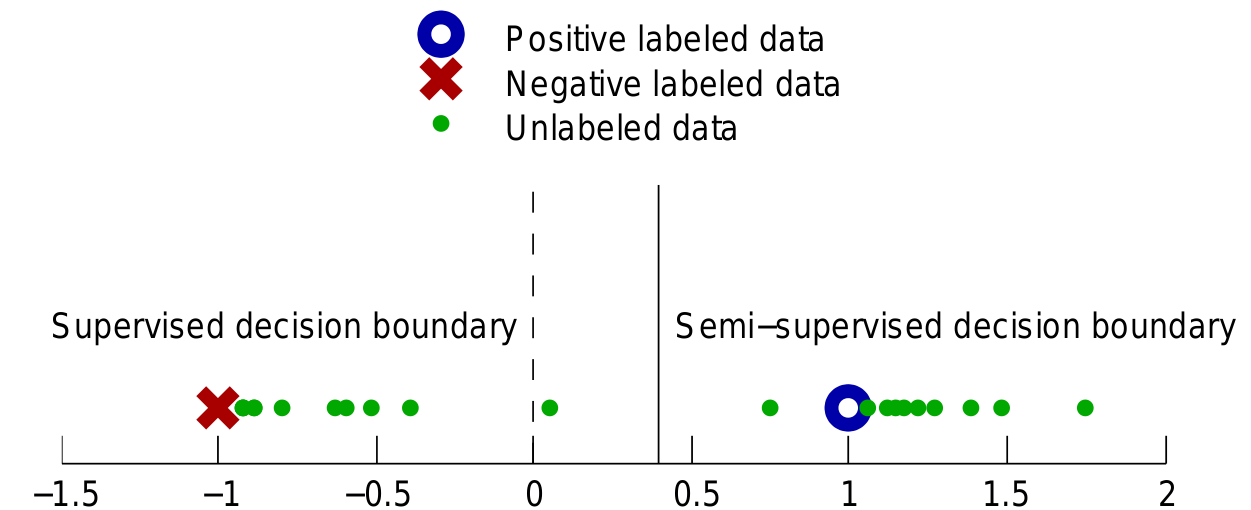
\includegraphics[width=.45\textwidth]{ssl-help}
  \end{center}
  \caption{Dados não-rotulados auxiliando a criar uma melhor fronteira de decisão. Fonte: \cite{zhu1}.}
  \label{fig:help}
\end{figure}

\begin{figure}[!h]
  \begin{center}
    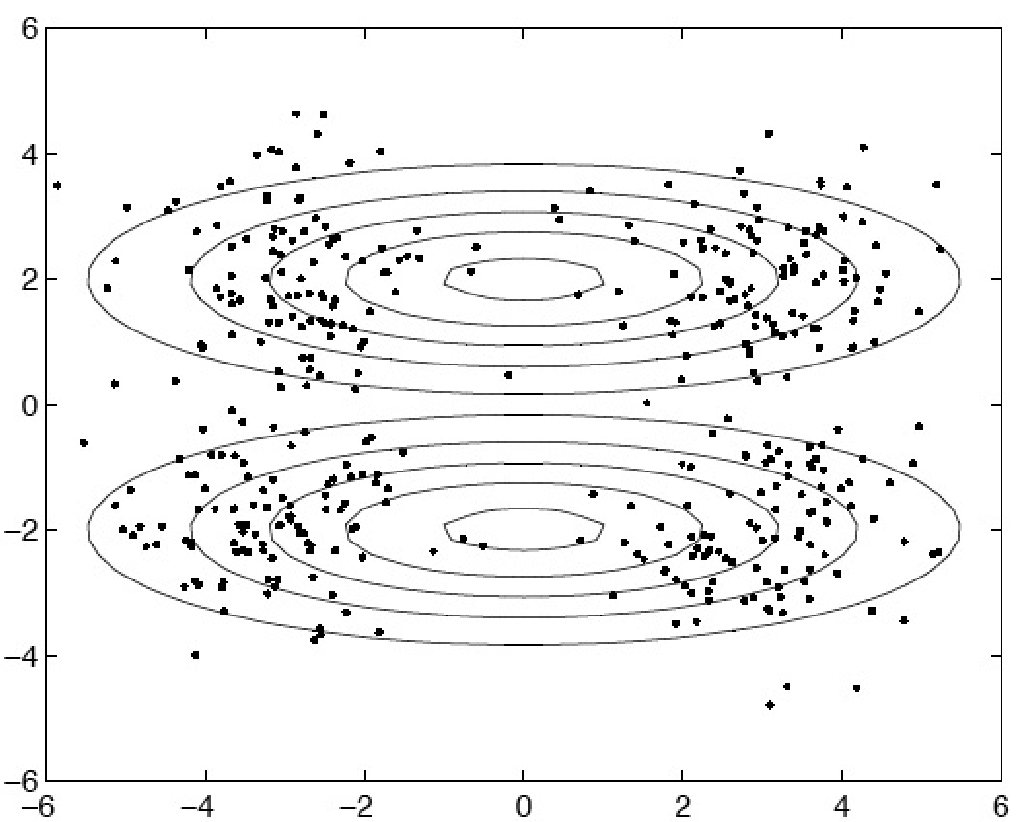
\includegraphics[width=.45\textwidth]{ssl-nhelp}
  \end{center}
  \caption{Dados não-rotulados atrapalhariam a correta separação das classes. Fonte: \cite{tub2008}.}
  \label{fig:nhelp}
\end{figure}


\subsubsection{Breve Histórico do Aprendizado Semi-Supervisionado}
Os primeiros trabalhos em CSS assumiam duas classes, cada uma com uma distribuição normal. Desta forma, os dados como um todo resultam em um \emph{modelo de mistura} (\emph{mixture model}). São necessárias somente de duas amostras rotuladas, uma de cada classe, para determinar completamente o modelo de mistura.

Uma variante é o \emph{self-training}: o classificador é treinado com os dados rotulados e depois aplicado aos não rotulados. Os pontos não rotulados que foram rotulados de forma mais confiante, são então adicionados ao conjunto de dados rotulados e então o classificador é treinado novamente. Este procedimento é chamado também de \emph{self-teaching} e \emph{bootstrapping}.

Ambos estes métodos são utilizados há muito tempo e continuam comuns devido à sua simplicidade conceitual e algorítmica.

Métodos mais recentes incluem o \emph{co-training} (em que dois classificadores utilizam partes disjuntas dos atributos de cada objeto e utiliza os novos objetos rotulados um do outro) e \emph{SVM transdutivo}.

Na última década, o aprendizado semi-supervisionado baseado em grafos atraiu grande atenção. Estes métodos iniciam-se com grafos cujos nós são os objetos rotulados e não rotulados e cujas arestas tem pesos que refletem a similaridade entre os objetos. Assume-se que objetos conectados por arestas de peso alto tendem a ter o mesmo rótulo e que os rótulos podem propagar-se pelo grafo. A seguir daremos uma definição e introdução mais formal sobre os grafos e sobre redes complexas.

\subsection{Grafos e Redes Complexas}
Está fora do escopo deste trabalho prolongar-se com a definição de grafos e redes complexas. Nesta parte é dado uma breve introdução e histórico sobre o tema. O estudo dos grafos é matéria da \emph{teoria dos grafos}.

Dito de forma direta, um grafo é uma representação abstrata de um conjunto de objetos no qual alguns destes objetos são ligados. Tais objetos são geralmente chamados de \emph{nós} ou \emph{vértices}. As ligações entre vértices são comumente chamadas de \emph{arestas}. Tipicamente, um grafo é visualmente representado por um conjunto de pontos ou bolas (os vértices) ligados por linhas (arestas).

Embora uma grande parte da teoria dos grafos seja elaborada apenas sobre esta estrutura básica descrita acima, existem diversos possíveis acréscimos estruturais. Provavelmente o mais importante é o de especificar uma direção para as arestas, resultando em \emph{arestas direcionadas}. A segunda característica diferencial de alguns grafos é a existência grandezas numéricas associadas às arestas, que resultam nas chamadas \emph{arestas com pesos}.

Outras características dos grafos são: mais de um tipo de aresta (possibilitando mais de uma aresta entre cada par de vértices); pesos associados aos nós; atributos diversos associados às arestas e aos nós (p.ex. cor); arestas incompletas; qualquer mistura de todas as características mencionadas acima.

Alguns grafos são clássicos, citamos alguns deles. Grafo regular é aquele no qual cada vértice tem o mesmo número de arestas. O grafo completo possui aresta entre qualquer par de vértices e também é chamado de \emph{click}. Um grafo conectado é aquele que apresenta um caminho de sucessão de arestas entre qualquer par de vértices. Grafo randômico é um grafo construído com uma probabilidade de se ter uma aresta entre dois vértices. Similarmente, um grafo randômico é aquele que exibe \emph{as mesmas características} que um grafo construído desta forma.

Formalmente falando, um grafo é um par ordenado $G=(V,E)$ composto de um conjunto de vértices $V$ e um conjunto $E$ de arestas, que são subconjuntos de $V$ com dois elementos. Estes são os grafos simples (com somente uma aresta possível entre cada par de vértices e sem aresta entre um vértice e ele mesmo) e não direcionado. Caso o conjunto $E$ seja composto de pares ordenados de elementos de $V$, o grafo é direcionado.

A medida mais comum de um grafo é o \emph{grau}, que é a quantidade de arestas ligadas a um vértice. Caso o grafo seja direcionado, podemos dividir o grau em duas quantidades: grau de entrada e grau de saída de um vértice. Caso o grafo tenha arestas com peso, pode-se falar em \emph{força} de um vértice que é a soma dos pesos das arestas ligadas ao vértice. Similarmente, podemos num grafo direcionado com peso, falar em força de entrada e força de saída de um vértice.

Antes de continuar com as medidas de um grafo, para o nosso caso é pertinente citar o que é uma \emph{rede complexa}. Dito de forma direta, uma rede complexa é um grafo com uma grande quantidade de vértices e arestas. Muitos pequisadores definem as redes complexas como sendo grafos de grandes dimensões que exibem características não triviais, isto é, que diferem de um grafo regular ou randômico. Esta definição é invalidada pelo fato de que se fala em rede complexa randômica e em rede complexa regular. Pode-se sim entender que a área de estudo das redes complexas se interessa pelos casos de redes complexas (comumente) encontrados na natureza que exibem características não triviais. 

Outra diferença entre as áreas de grafo e redes complexas é que enquanto a área de grafos tradicionalmente é vinculada à extração de propriedades matemáticas de grafos em geral ou com construções particulares, a área de redes complexas é marcada mais acentuadamente pela observação das redes complexas que representam fenômenos humanos ou naturais e suas divergências se comparadas às redes mais triviais (regulares e randômicas). Exemplos destas características peculiares são as conhecidas \emph{lei livre de escala} e \emph{lei de pequeno mundo}.

\subsubsection{Breve Histórico da Teoria dos Grafos e das Redes Complexas}
A estrutura de pontos e retas é tão simples que é difícil precisar quando foi utilizada pela primeira vez, se é que isso é possível. O artigo escrito por Leonhard Euler chamado "Konigsberg Bridge problem" é geralmente descrito como o primeiro trabalho tanto de topologia quanto de teoria dos grafos.

Mais de um século depois, Cayley estudou \emph{árvores} através de formas analíticas que surgiam do cálculo diferencial. Tais estudos tiveram grandes consequências para a química teórica e esta fusão entre química e grafos está no centro da nomenclatura comum utilizada para grafos.

Em particular, o nome \emph{grafo} foi introduzido por Sylvester em 1878 através de um artigo publicado na Nature.

No século XX a teoria dos grafos teve focos diferentes, passando pelo problema de coloração de grafos, topologia (em particular em conexão com a álgebra, p.ex. \emph{Lei de Kirchoff} para circuitos), e, por fim, por teorias probabilísticas.

Já adentrando o terreno das chamadas redes complexas, os artigos que demonstravam as características \emph{livre de escala} e de \emph{pequeno mundo} para grafos grandes representando estruturas da natureza~\cite{ferrer,barabasi} marcaram este novo grande interesse pela área.

Atualmente, as redes complexas são aplicadas com sucesso a diversas áreas~\cite{costaapp}, o que inclui neurociências~\cite{sporns}, física~\cite{pnas}, linguística~\cite{dorogo2} e ciência da computação~\cite{signature}, para citar simplesmente alguns casos.


\subsection{Aprendizado Semi-Supervisionado em Grafos}
Diversas técnicas de CSS baseada em grafos tem sido desenvolvidas e utilizadas. Citamos os seguintes métodos, de forma ilustrativa e sem a pretensão de obtermos uma lista completa: algorítmo de regularização ~\cite{reg}, mincut ~\cite{mincuts}, propagação de rótulo ~\cite{zhu3}, modelos de mistura e maximização de entropia \cite{zhu1}.

De especial importância é a forma de construção do grafo. Uma discussão detalhada sobre o assunto é encontrada no terceiro capítulo de ~\cite{zhu1}.

Para um detalhamento das técnicas \emph{mincut} e \emph{propagação de rótulo} nos referimos ao outro trabalho apresentado nesta disciplina ~\cite{sslgraph}. Cabe lembrarmos aqui que, dadas as convenções envolvidas e explicitadas no referido artigo, a técnica de propagação de rótulo pode ser entendida pela seguinte fórmula:

\begin{equation}
  f_u = (I - P_{UU})^{-1}P_{UL}Y_{L}
\end{equation}

Isso nos permite resolver a propagação de rótulo diretamente sem a propagação iterativa.


\section{Material e Métodos}
\subsection{Redes de Palavras}
\subsubsection{Regra de Formação}

\begin{table}
\centering
\caption{Pré-processamento da sentença ``The projection of the dataset into three dimensions is essential for very large datasets''. Note que as \emph{stopwords} são removidas e as palavras restantes são lematizadas.}
\label{tab:a0}       % Give a unique label
\begin{tabular}{p{3.5cm}p{3.5cm}}
\hline\noalign{\smallskip}
Original sentence & Pre-processed sentence    \\
\noalign{\smallskip}\svhline\noalign{\smallskip}
{\small The projection of the dataset} 			& {\small projection dataset}\\
{\small into three dimensions is essential} 		& {\small three dimension be essential}\\
{\small for very large datasets}						& {\small very large dataset}\\
\noalign{\smallskip}\hline\noalign{\smallskip}
\end{tabular}
\end{table}

O método utilizado consiste em duas partes. A primeira é o processamento das palavras através da remoção das chamadas \emph{stopwords} e de toda pontuação do texto. Em sequência efetuamos a lematização das palavras restantes. Tal procedimento pode ser visualizado na Figura \ref{tab:a0}.


\begin{figure}[t]
%\sidecaption[t]
% Use the relevant command for your figure-insertion program
% to insert the figure file.
% For example, with the option graphics use
\begin{center}
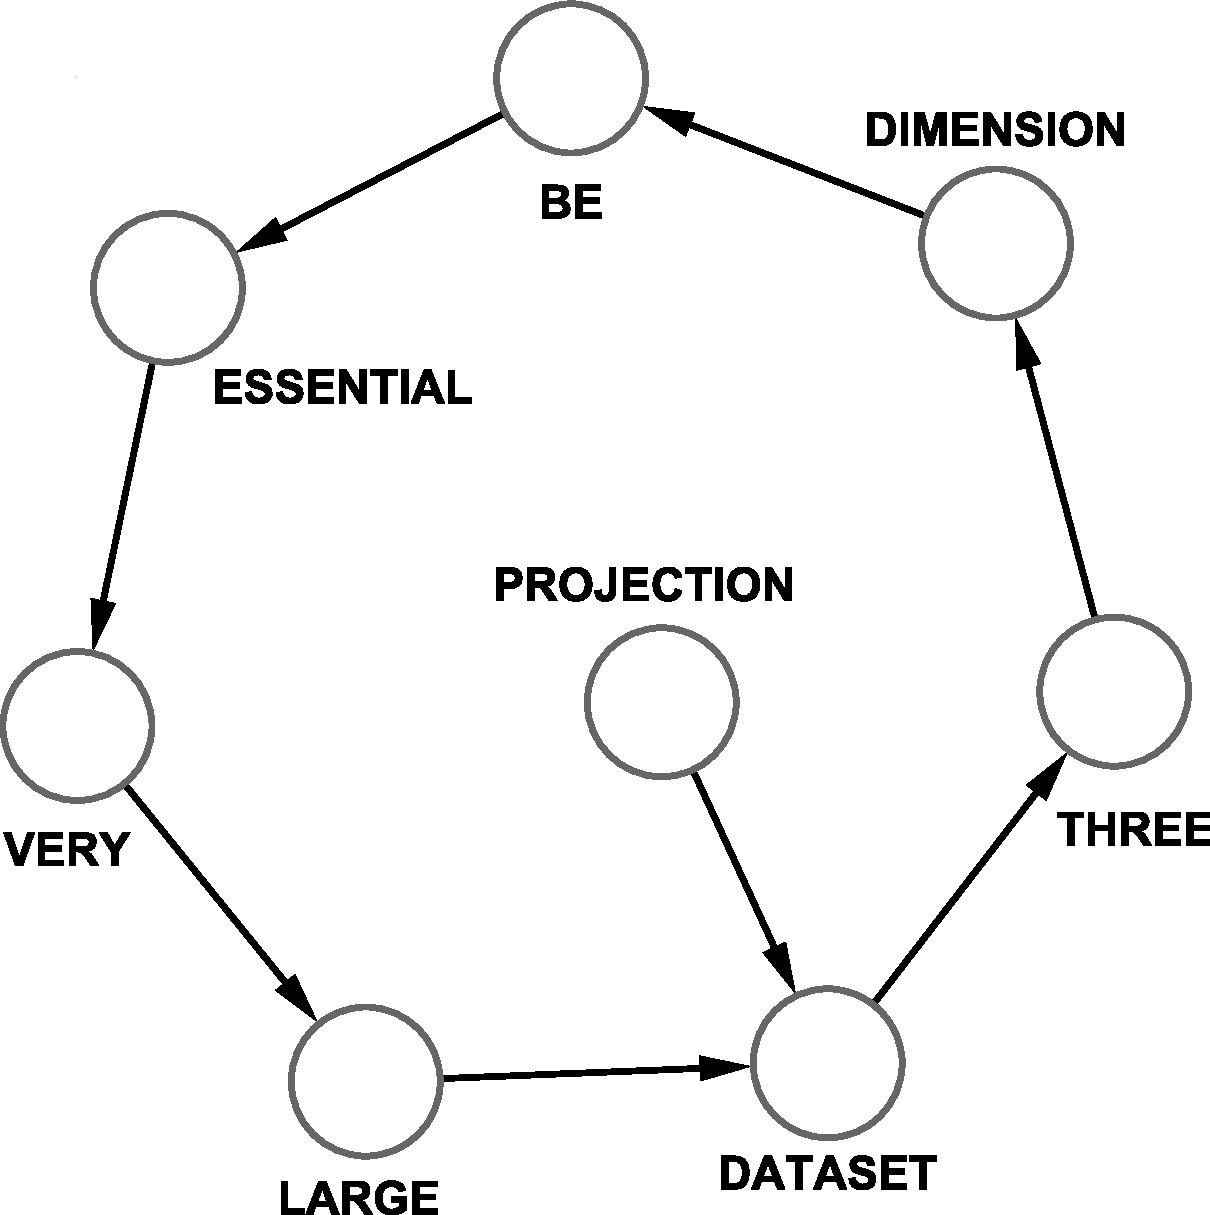
\includegraphics[scale=.27]{data}
\end{center}
%
% If no graphics program available, insert a blank space i.e. use
%\picplace{5cm}{2cm} % Give the correct figure height and width in cm
%
%\caption{Please write your figure caption here}
\caption{Exemplo de formação de rede resultante da senteça ``The projection of the dataset into three dimensions is essential for very large datasets''.}
\label{fig:r0}       % Give a unique label
\end{figure}

 A segunda parte da formação da rede consiste em tomar cada palavra como um vértice e em estabelecer arestas entre palavras consecutivas. Quando uma mesma palavra é encontrada novamente, ela é entendida como o mesmo vértice. Este procedimento pode ser visto na Figura \ref{fig:r0}. Sabe-se que redes complexas assim formadas são do tipo livre de escala e pequeno mundo.


\subsubsection{Formação das Redes de Palavras}
O corpus utilizado consiste em textos da Folha de São Paulo coletados durante dez anos. A seção do citado jornal do qual foram coletados os textos consistia em uma opinião positiva e outra negativa a respeito de determinado assunto.

Os textos foram divididos entre positivos e negativos. Em cada grupo, redes eram formadas aglomerando-se os textos até atingirem 1200 vértices. Como resultado obtemos diversas redes com 1200 vértices, cada rede formada somente por textos positivos ou negativos. Obtivemos 50 redes positivas e 50 redes negativas.

Na sequência realizamos as seguintes medidas: graus, coeficientes de clusterização, caminhos mais curtos, eficiência global, proximidade(closeness) e acessibilidade. Com cada uma destas medidas foram obtidas a média, desvio padrão, mediana e quartis.


\subsection{Processamento de Fala}
Na seção 2.2 foram expostas as diferentes medidas usuais para o processamento de fala. Em nosso caso, utilizamos somente medidas de frequência fundamental. Utilizando o programa livre Praat ~\cite{praat} e scripts próprios em Praat e Python, realizamos medidas de frequência fundamental a cada 10 milisegundos nos arquivos de áudio envolvidos.

\subsubsection{Arquivos de Áudio e Medidas Derivadas da Sucessão de Frequências Fundamentais}
Foram utilizados cinquenta trechos de fala de duração livre entre três e sete segundos. Todos foram retirados de um mesmo depoimento encontrado no projeto Iboruna ~\cite{iboruna}. Metade dos trechos foram trechos que, quando ouvidos no depoimento original, foram tidos como positivos. A outra metade são trechos que quando ouvidos foram classificados como negativos. Isso segundo um único ouvinte, ou seja, os dados são de um único locutor e classificados segundo a paercepção de uma única pessoa (o autor deste trabalho).

Para cada arquivo, foi efetuada as seguintes medidas sobre a sequência de frequências fundamentais: média, desvio padrão, âmbito, mediana, porcentagem de medições dentre as localizadas no quinto inferior do âmbito, porcentagem de medições dentre as localizadas no quinto superior do âmbito.

\section{Resultados}
\subsection{Redes de Palavras}
Escolhemos 50\% das redes para treinamento. Cada vez que os algorítmos eram rodados, as redes eram escolhidas ao acaso. O treinamento semi-supervisionado por propagação de rótulos deu a maior variação entre cada rodada, atingindo marcas de 80\% de acerto. Na média, conseguimos um ganho de 2-3\% em relação aos métodos usuais que utilizamos. O resultado está sumarizado nas Tabelas \ref{tab:4rec} e \ref{tab:prerec}. 

\begin{table}
\centering
\caption{\% de textos classificados corretamente. O melhor classificador foi o de propagação de rótulos com 67,65 \% de acerto (na média).} 
\label{tab:4rec}       % Give a unique label
\begin{tabular}{p{4.5cm}p{2cm}}
\hline\noalign{\smallskip}
Método & Acerto    \\
\noalign{\smallskip}\svhline\noalign{\smallskip}
Bayesian Decision & 60,39 \%\\
Decision Tree & 61,27 \%\\
Decision Rules & 64,08 \%\\
Naive Bayes & 64,79 \%\\
Propagação de Rótulos & 67,65 \%\\
\noalign{\smallskip}\hline\noalign{\smallskip}
\end{tabular}
\end{table}

\begin{table}
\centering
\caption{Precisão e Cobertura para opiniões positivas e negativas.}
\label{tab:prerec}       % Give a unique label
\begin{tabular}{p{1.5cm}p{1cm}p{1cm}p{1cm}p{1cm}}
\hline\noalign{\smallskip}
{\footnotesize Método} & {\footnotesize Precisão Pos.} & {\footnotesize Cobertura Pos.} & {\footnotesize Precisão Neg.} & {\footnotesize Cobertura Neg.} \\
\noalign{\smallskip}\svhline\noalign{\smallskip}
{\footnotesize Bayesian Decision} & {\footnotesize 70,2} \%  & {\footnotesize 49,3} \% & {\footnotesize 77,3} \% & {\footnotesize 71,4 \%} \\
{\footnotesize Decision Tree} &  {\footnotesize 71,1} \% & {\footnotesize 38,0} \% & {\footnotesize 57,7} \% & {\footnotesize 84,5} \% \\
{\footnotesize Decision Rules} & {\footnotesize 70,0} \% & {\footnotesize 49,3} \% & {\footnotesize 60,9} \% & {\footnotesize 78,9} \% \\
{\footnotesize Naive Bayes} & {\footnotesize 70,6} \% & {\footnotesize 50,7} \% & {\footnotesize 61,5} \% & {\footnotesize 78,9} \% \\
{\footnotesize Propagação de Rótulo} & {\footnotesize 60,0} \% & {\footnotesize 83,3} \% & {\footnotesize 72,7} \% & {\footnotesize 44,4} \% \\
\noalign{\smallskip}\hline\noalign{\smallskip}
\end{tabular}
\end{table}


\subsection{Trechos de Fala}
Escolhemos também 50\% das redes para treinamento. Cada vez que os algorítmos eram rodados, as redes eram escolhidas ao acaso. Aqui houve grande surpresa, com um aumento de 20\% nas classificações corretas. Os resultados estão sumarizados nas Tabelas \ref{tab:5rec} e \ref{tab:preerec}.

\begin{table}
\centering
\caption{\% de textos classificados corretamente. O melhor classificador foi o de propagação de rótulos com 67,65 \% de acerto (na média).} 
\label{tab:5rec}       % Give a unique label
\begin{tabular}{p{4.5cm}p{2cm}}
\hline\noalign{\smallskip}
Método & Taxa de Acerto    \\
\noalign{\smallskip}\svhline\noalign{\smallskip}
RIP & 57,78 \%\\
Naive Bayes & 53,33 \%\\
Propagação de Rótulos & 75,71 \%\\
\noalign{\smallskip}\hline\noalign{\smallskip}
\end{tabular}
\end{table}

\begin{table}
\centering
\caption{Precisão e Cobertura para opiniões positivas e negativas.}
\label{tab:preerec}       % Give a unique label
\begin{tabular}{p{1.5cm}p{1cm}p{1cm}p{1cm}p{1cm}}
\hline\noalign{\smallskip}
{\footnotesize Método} & {\footnotesize Precisão Pos.} & {\footnotesize Cobertura Pos.} & {\footnotesize Precisão Neg.} & {\footnotesize Cobertura Neg.} \\
\noalign{\smallskip}\svhline\noalign{\smallskip}
{\footnotesize RIP} & {\footnotesize 52,4 \%}  & {\footnotesize 55,0 \%} & {\footnotesize 62,5 \%} & {\footnotesize 60,0 \%} \\
{\footnotesize Naive Bayes} & {\footnotesize 47,1 \%} & {\footnotesize 40,0 \%} & {\footnotesize 57,1 \%} & {\footnotesize 64,0 \%} \\
{\footnotesize Propagação de Rótulo} & {\footnotesize 66,6 \%} & {\footnotesize 80,0 \%} & {\footnotesize 83,3 \%} & {\footnotesize 71,4 \%} \\
\noalign{\smallskip}\hline\noalign{\smallskip}
\end{tabular}
\end{table}


\section{Conclusão}
Embora na literatura seja bastante enfatizado que a utilização de dados não rotulados para algoritmos de aprendizado de máquina é de grande utilidade quando os dados rotulados são poucos ou custosos, mostramos a utilidade do algorítmo de propagração de rótulos para dois casos diferentes em que os objetos rotulados eram metade dos objetos. Isso tanto desmistificou o uso do aprendizado semi-supervisionado para o caso de uma grande quantidade de objetos rotulados que os testes com poucos objetos rotulados não chamou atenção e foi inclusive omitido deste trabalho.

Dada a supresa, estamos começando já a utilizar o método de propagação de rótulos nas pesquisas que estamos realizando no grupo. Os próximos passos são claramente conseguir mais exemplos para atigir resultados mais relevantes. É necessário obter mais trechos e analizar fala de outros locutores.

Outra via que queremos explorar e que tem com os conteúdos desenvolvidos nesta disciplina é a utilização de redes formadas a partir das sequências de medidas das falas. Desenvolvemos um método de criação de redes que exibe lei livre de escala para a distribuição de grau dos vértices. Também estamos estudando redes criadas pelo método conhecido como \emph{redes de visibilidade}. Há ainda um terceiro método, este não explorado, que constrói a rede a partir da matriz de correlação relacionada à série temporal de origem.

A disponibilização dos algoritmos na rede\footnote{svn co http://svn.assembla.com/svn/audioexperiments} permite não só a troca facilitada de conhecimentos e tecnologias, mas também que possamos acessar o algoritmo de qualquer lugar. Esta disponibilidade também nos incentiva a arrumar o código de forma a deixá-lo facilmente utilizável.

\begin{thebibliography}{}


\bibitem[\protect\citename{Gonçalves, S. C. L.}]{iboruna}
Gonçalves, S. C. L.
\newblock {Banco de dados Iboruna: amostras eletrônicas do português falado no interior paulista.}.
\newblock {\em http:://www.alip.ibilce.unesp.br/iboruna. }.

\bibitem[\protect\citename{Zhu, X. and Lafferty, J. and Rosenfeld, R.}2005]{zhu1}
Zhu, X. and Lafferty, J. and Rosenfeld, R.
\newblock 2005.
\newblock {Semi-supervised learning with graphs}.
\newblock {\em Unpublished doctoral dissertation}.

\bibitem[\protect\citename{Zhu, X.}2007]{zhu2}
Zhu, X.
\newblock 2006.
\newblock {Semi-supervised learning literature survey}.
\newblock {\em Citeseer}.

\bibitem[\protect\citename{Zhu, X. and Ghahramani, Z.}2003]{zhu3}
Zhu, X. and Ghahramani, Z.
\newblock 2002.
\newblock {Learning from labeled and unlabeled data with label propagation}.
\newblock {\em Citeseer}.

\bibitem[\protect\citename{Blum, A. and Chawla, S.}2001]{mincuts}
Blum, A. and Chawla, S.
\newblock 2001.
\newblock {Learning from labeled and unlabeled data using graph mincuts}.

\bibitem[\protect\citename{Belkin, M. and Matveeva, I. and Niyogi, P.}2004]{ferrer}
Belkin, M. and Matveeva, I. and Niyogi, P.
\newblock 2004.
\newblock {Regularization and Semi-supervised Learning on Large Graphs}.
% \newblock {\em Proceedings of the Royal Society of London B}, 268:2261.

\bibitem[\protect\citename{Müller, K. R. and Zien, A.}2008]{tub2008}
Müller, K. R. and Zien, A.
\newblock 2008.
\newblock {Semi-Supervised Learning}.

\bibitem[\protect\citename{Chapelle, O. and Sch{\\"o}lkopf, B. and Zien, A.}2006]{sslbook}
Chapelle, O. and Sch{\\"o}lkopf, B. and Zien, A.
\newblock 2006.
\newblock {Semi-supervised learning}.
\newblock {\em Citeseer}.

\bibitem[\protect\citename{Boersma, P. and Weenink, D.}2010]{praat}
Boersma, P. and Weenink, D.
\newblock 2010.
\newblock {Praat: doing phonetics by computer [Computer program]}.
\newblock {\em http://www.praat.org/}.

\bibitem[\protect\citename{Ferrer i Cancho and Sole}2001]{ferrer}
R. Ferrer i Cancho and R. V. Sole.
\newblock 2001.
\newblock {The small world of human language}.
\newblock {\em Proceedings of the Royal Society of London B}, 268:2261.

\bibitem[\protect\citename{Newman}2003]{newman}
M. E. J. Newman. 
\newblock 2003.
\newblock {The Structure and Function of Complex Networks}.
\newblock {\em SIAM Review}, 45:167--256.

\bibitem[\protect\citename{Albert and Barabasi}2002]{barabasi}
R. Z. Albert and A.L. Barabasi. 
\newblock 2002.
\newblock {Statistical Mechanics of Complex Networks}.
\newblock {\em Rev. Modern Phys.}, 74:47--97.

\bibitem[\protect\citename{Costa \bgroup et al.}2008]{costaapp}
L. F. da Costa, O. N. Oliveira Jr., G. Travieso, F. A. Rodrigues, P. R. Villas Boas, L. Antiqueira, M. P. Viana, L. E. C. da Rocha. 
\newblock 2008.
\newblock {Analyzing and Modeling Real-World Phenomena with Complex Networks: A Survey of Applications}.
\newblock {\em arXiv} 0711.3199.

\bibitem[\protect\citename{Sporns}2002]{sporns}
O. Sporns. 
\newblock 2002.
\newblock {Network analysis, complexity, and brain function}.
\newblock {\em Complexity}, 8(1):56--60.

\bibitem[\protect\citename{Gfeller}2007]{pnas}
D. Gfeller, P. LosRios, A. Caflisch and F. Rao.
\newblock 2007.
\newblock {Complex network analysis of free-energy landscapes}.
\newblock {\em Proceedings of the National Academy of Science USA}, 104 (6):1817--1822

\bibitem[\protect\citename{Dorogovtsev and Mendes}2001]{dorogo2}
S. N. Dorogovtsev and J. F. F.Mendes.
\newblock 2001.
\newblock {Language as an evolving word web}.
\newblock {\em Proceedings of the Royal Society of London B}, 268:2603.

\bibitem[\protect\citename{Moura \bgroup et al.}2003]{signature}
A. P. S. de Moura, Y. C. Lai and A. E. Motter.
\newblock 2003.
\newblock {Signatures of small-world and scale-free properties in large computer programs}.
\newblock {\em Physical Review E}, 68(1):017102.

\bibitem[\protect\citename{Belkin, M. and Matveeva, I. and Niyogi, P.}2004]{reg}
Belkin, M. and Matveeva, I. and Niyogi, P..
\newblock 2004.
\newblock {Regularization and semi-supervised learning on large graphs}.
\newblock {\em Learning theory, Springer}, 624--638.

\bibitem[\protect\citename{Jusczyk, P. W. }2000]{spkl}
Jusczyk, P. W. 
\newblock 2000.
\newblock {The Discovery of Spoken Language}.
\newblock {\em The MIT Press}.

\bibitem[\protect\citename{Teixeira, A.}2009]{flem}
Teixeira, A.
\newblock 2009.
\newblock {Fala e Emoção}.
\newblock {\em Tese de Doutoramento, Universidade de Aveiro}.

\bibitem[\protect\citename{McLuhan, M.}1962]{guten}
McLuhan, M.
\newblock 1962.
\newblock {The Gutenberg Galaxy: The Making of Typographic Man}.
\newblock {\em University of Toronto Press}.


\bibitem[\protect\citename{Borges, C. de A.}2004]{teatro}
Borges, C. de A.
\newblock 2004.
\newblock {Dando corpo a palavra : um exercicio cenico sobre a voz}.
\newblock {\em Tese de Mestrado, Universidade de Campinas}.

\bibitem[\protect\citename{Dalgalarrondo, P.}2008]{dalga}
Dalgalarrondo, P.
\newblock 2008.
\newblock {Psicopatologia e Semiologia dos Transtornos Mentais}.
\newblock {\em Artmed}.

\bibitem[\protect\citename{Yacoub, S. and Simske, S. and Lin, X., and Burns, J.}2003]{interactivevoice}
Yacoub, S. and Simske, S. and Lin, X., and Burns, J.
\newblock 2003.
\newblock {Recognition of emotions in interactive voice response systems}.
\newblock {\em Eighth European conference on speech communication and technology}.

\bibitem[\protect\citename{Tóth, S. L. and Sztahó, D. and Vicsi, K.}]{humanmachine}
Tóth, S. L. and Sztahó, D. and Vicsi, K.
\newblock {Speech Emotion Perception by Human and Machine}.
\newblock {\em Verbal and Nonverbal Features of Human-Human and Human-Machine Interaction. LNCS (LNAI), Volume 5042, p. 213-224.}.

\bibitem[\protect\citename{McGilloway, S. and Cowie, R. and Douglas-Cowie, E. and Gielen, S. and Westerdijk, M. and Stroeve, S.}2000]{benchmark}
McGilloway, S. and Cowie, R. and Douglas-Cowie, E. and Gielen, S. and Westerdijk, M. and Stroeve, S.
\newblock 2000
\newblock {Approaching automatic recognition of emotion from voice: a rough benchmark}.
\newblock {\em ISCA Tutorial and Research Workshop (ITRW) on Speech and Emotion}.

\bibitem[\protect\citename{Fabbri, R.}2010]{sslgraph}
Fabbri, R.
\newblock 2010
\newblock {Aprendizado Semi-Supervisionado Baseado em Grafos}.
\newblock {\em Trabalho da matéria Matéria SCC5882 sob orientação dos Profs. Dr. Zhao Liang e Dr. Alneu de Andrade Lopes}.

\bibitem[\protect\citename{Toivanen, J. and Seppänen, T. and Väyrynen, E.}2009]{autoreview}
Toivanen, J. and Seppänen, T. and Väyrynen, E.
\newblock 2009
\newblock {Automatic Discrimination of Emotion from Voice: A Review of Research Paradigms}.
\newblock {\em Emotions in the Human Voice, v. 3, cap. 5, p. 67-78}.

\bibitem[\protect\citename{Sidarova, J. and McDonough, J. and Badia, T.}2009]{autoemotive}
Sidarova, J. and McDonough, J. and Badia, T.
\newblock 2009
\newblock {Automatic Recognition of emotive Voice and Speech}.
\newblock {\em Emotions in the Human Voice, v. 3, cap. 12, p. 205-237}.


\bibitem[\protect\citename{Bird, S. and Klein, E. and Loper, E.}2009]{livro-nltk}
Bird, S. and Klein, E. and Loper, E.
\newblock 2009
\newblock {Natural Language Processing with Python}.
\newblock {\em O'Reilly Media}.

\bibitem[\protect\citename{Jurafsky, D. and Martin, J. H.}2000]{Jurafsky}
Jurafsky, D. and Martin, J. H.
\newblock 2000
\newblock {Speech and Language Processing: An Introduction to Natural Language Processing Computational Linguistics}.
\newblock {\em Prentice Hall}.

% \bibitem[\protect\citename{John and Langley}1995]{bayes}
% G. H. John and P. Langley.
% \newblock 1995.
% \newblock {Estimating Continuous Distribution in Bayesian Classifiers}.
% \newblock {\em 11 Conference on Uncertainty in Artificial Intelligence}, 338--345. 
% 
% \bibitem[\protect\citename{Kohavi}1995]{cross}
% R. Kohavi.
% \newblock 1995.
% \newblock {A study of cross-validation and bootstrap for accuracy estimation and model selection}.
% \newblock {\em Proceedings of the Fourteenth International Joint Conference on Artificial Intelligence 2}, 12:1137-1143. 

\end{thebibliography}

\end{document}







